\section{FreeRTOS}
\note{Kort intro til hvad FreeRTOS er og hvilken funktionalitet det stiller tilrådighed}
Som indlejret styresystem benyttes FreeRTOS. 
FreeRTOS er et open source real-tids styresystem til indlejrede systemer, som er blevet en industriel standard. 
Styresystemet er valgt, da det er simpelt at gå til. 
Det er desuden primært skrevet i programmeringssproget C, som også benyttes i projektet. 
FreeRTOS benytter preemptive schedulering til at administrere CPU-tiden mellem tasks. 

\section{Preemptive schedulering}
FreeRTOS er bygget på en prioritetsbaseret preemptive scheduleringsalgoritme.\newline
Når et operativ system opererer med en preemptive scheduleringsalgoritme kan kørende processer preemptes - blive stoppet - og skiftet ud med en anden proces.\newline
Det kan f.eks. være at en proces der har ventet på en I/O device får tilgang til denne.
Scheduleren vil så skifte den nuværende kørende proces ud og skifte den hidtil ventende proces ind så den kan køres.
Dette gør scheduleren via et context switch.\newline
Når et context switch sker gemmes ''konteksten`` af den nuværende task i en process control block (PCB), og ydermere sker der et state restore, hvor informationen i PCBen af den task, der skal skiftes til hentes.
Det som bliver gemt i PCBen er værdierne i CPU registrene (Program counter, etc.) og anden vigtig operativ systemsinformation.\newline
Prioritetsbaseret skeduleringsalgoritmer tildeler alle tasks en prioritet som er baseret på taskens vigtighed.\newline
FreeRTOS er et real-time operativ system og et primært formål ved real-time operativ systemer er at give et respons på begivenheder indenfor en vis deadline.
FreeRTOS skeduleringsalgoritme sørger så for at den task med højest prioritet bliver givet processortid.

\note{afsnit om task, task model, hid queues og implementering i os}

\section{Interrupt håndtering}
\note{Interrupt execution diagram og opsætning} 
\subsection{Intterrupt eksekvering og task skedulering}
\label{subsec:int_task}
Figur \ref{fig:int_task} viser hvordan tasks og interrupts håndteres i FreeRTOS. 
Til tiden t1 kører en lavt prioriteret task. 
Ved t2 bliver en interrupt service rutine, fremover kaldet en ISR, kaldt. 
Den prioriteres højest, og den lavt prioriteret task pauses indtil ISR'en er færdig.
ISR'eren er færdig til tiden t3, hvor den lavt prioriteret task kan genoptages.
Ved t4 sker et context switch til en højere prioriteret task.
Skeduleringen mellem tasks er styret af FreeRTOS scheduler med respekt til den prioritet, som hver task er givet. 
Interrupts prioriteres højere end alle tasks, uanset prioriteten af den pågældende task. 
Interrupts har også prioriteter i mellem sig, såfremt flere skulle blive kaldt. 
Modsat tasks, vil en interrupt dog altid afsluttes, før den næste kan begynde. 
ARM Cortex-M4 tilbyder otte interrupt prioriteter. 
\husk{Jes}{Forstået rigtigt?} 
\begin{figure}[h]
	\caption{Det tidslige forløb for to tasks og en interrupt service rutine. }
	\centering
	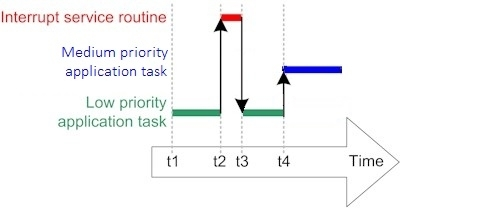
\includegraphics[width=0.6\linewidth]{billeder/interruptandtaskprocessing.jpg}
	\label{fig:int_task}
\end{figure}

Når det indgående lydsignal skal samples gennem ADC'en, skal samplingen foregå periodisk på nøjagtigt det samme tidspunkt i hver periode.
Det faste tidspunkt for sampling giver minimal jitter med en minimal forsinkelse i samplingen af signalet. 
\husk{Jes}{Dansk ord for jitter? Det er et teknisk engelsk ord, så det kan vel gå.. } 
For at sikre, at mikrocontrolleren sætter alle andre opgaver på pause, og begynder at sample på det korrekte tidspunkt, implementeres samplingen i en ISR.

\subsection{Implementering af interrupt-styring med timer}
\label{subsec:impl_int}
ISR'en indstilles med den højest mulige interrupt prioritet. 
Timingen af ISR'en er styret af Timer 3. 
Timeren er implementeret som en 16-bit timer i periodic timer mode, edge-count mode og inverted PWM mode.
Ved start hentes timerens start value ind i et tælleregister. 
Sample-frekvensen og CPU frekvensen styrer værdien. 
\begin{equation}
	\text{Timer start value register} = \frac{\text{CPU'ens frekvens}}{\text{Sample-frekvens}} = \frac{80\text{MHz}}{44,1\text{kHz}} \simeq 1814
\end{equation}
I periodic timer mode vil timeren dekrementere fra tælleregisteret, som automatisk henter timer start værdien igen, og begynder forfra når værdien når nul. 
Når værdien når nul, kaldes den ISR som sikrer at lydsignalet bliver samplet. \newline

\section{Sampling af lydsignal igennem ADC}
Microcontrolleren har to identiske ADC moduler, som opererer uafhængigt ad hinanden. 
De kan derfor sample på samme tidspunkt. 
ADC'erne er opbygget med Successive Approximation Register arkitektur, som leverer en opløsning på 12-bit, hvilket giver 4096 mulige steps i det digitale resultat. 
ADC'ens interne forsyningsspænding og ground er på henholdsvis 3,3V og 0V, hvilket samtidig er den maksimale og minimale spændingsreference, som ADC'en kan læse. 
Stepsizen er $\Delta$ er udregnet i formel \ref{eq:ADC_res}.
\begin{equation}
\label{eq:ADC_res}
	\Delta = \frac{X_{maks}-X_{min}}{steps} = \frac{3\text{V}-0\text{V}}{4096} = 0,73\text{mV}
\end{equation}
\husk{Jes}{Stepsize udregning kan måske udelades, hvis vi får pladsmangel.}
ADC'en er drevet af en 16MHz clock, og det tager 250ns at tage én sample. 

\subsection{Opsætning af ADC}
ADC0 og ADC1 er sat op til at modtage et analogt signal, for henholdsvis venstre og højre kanal, direkte på to general purpose input pins (GPIO). 
Start af sampling er indstillet, så det trigges af et processor event. 
Det betyder at en sampling i praksis startes ved at skrive til ADC Processor Sample Sequence Initiate registeret. 
Resultatet af en A/D konvertering, kan læses i sequence 3. 
ADC'en har fire individuelle sequence registre, som kan indeholde op til flere samples efter FIFO princippet. 
Sequence 3 er valgt, da den kun kan indeholde én sample, hvilket er praktisk når samplingens timing skal være præcis. 
Yderligere samples ville ikke være brugbare, fordi de ville være målt på et forkert tidspunkt. 

\subsection{ISR sample handler og ADC}
Som nævnt i afsnit \ref{subsec:int_task}, vil det timerstyrede interrupt kalde sample handler rutinen.
I rutinen startes samplingen som det allersidste. 
Det betyder at dataene fra samplingen bliver gemt i sequence 3 registeret indtil næste gang interruptet kaldes. 
Næste gang interruptet kaldes, gemmes dataene i en variabel, og en ny AD konvertering bliver herefter igen udført. 
Fordelen er at hver gang ISR'en bliver kaldt, vil samplen ligge klar.
Der skal ikke ventes på en konvertering. 
Det betyder også at forsinkelsen fra en konvertering bliver konstant. Forsinkelsen vil være givet ved $\frac{1}{f_s}$. 

\subsection{Offset og trunkering af samplet data}
Værdien af den modtagede sample fra AD konverteringen vil have et offset pga. DC forskydningen ved input stage, som tidligere beskrevet i afsnit \ref{sec:inputstage}.
Offsettet fjernes igen ved at trække $\frac{4096}{2} = 2048$ fra resultatet af AD konverteringen. 
Resultatet gemmes som en værdi af data typen float. 
\husk{Jes}{Skal vi have en graf, hvor man kan se at signalet flyttes?}
\husk{Jes}{Afsnit ikke færdigt!}
% Der sker noget mere.. 11 bit offset, trunkering og cast?

\subsection{Sample handler og processortid}
Da sample handleren kører periodisk, og i form af en ISR har højeste prioritet til processortid, skal alle andre processoropgaver foregå i al den mellemliggende tid. 
Det betyder at sample handleren og AD konverteringen skal være effektiv, således andre tasks kan nå at køre færdig, inden sample handleren kaldes igen. 
\husk{Jes}{Har vi mulighed for at kende den tid det tager rutinen at køre igennem? }
% tid per sample. Hvad kan nås osv.

\section{Modulær opbygning af effekter}
Da effekterne skal være modulær
Effektmodulerne bliver kaldt via 
Effektmodulerne holdes hver især i en \textit{module control block}, $\mathtt{mcb\_t}$,  som er en data struktur bestående af en \textit{function pointer} og en booleansk variabel.
Function pointeren benyttes til at kalde lydeffektmodulerne, og den booleanske variabel benyttes til at aktivere/deaktivere lydeffekterne.\newline
For at tilføje en lydeffekt laves der en ny instans af $\mathtt{mcb\_t}$, og dens \textit{function pointer} sættes til at \textit{pointe} til lydeffekt rutinen.\newline
\begin{figure}[!ht]
	\centering
	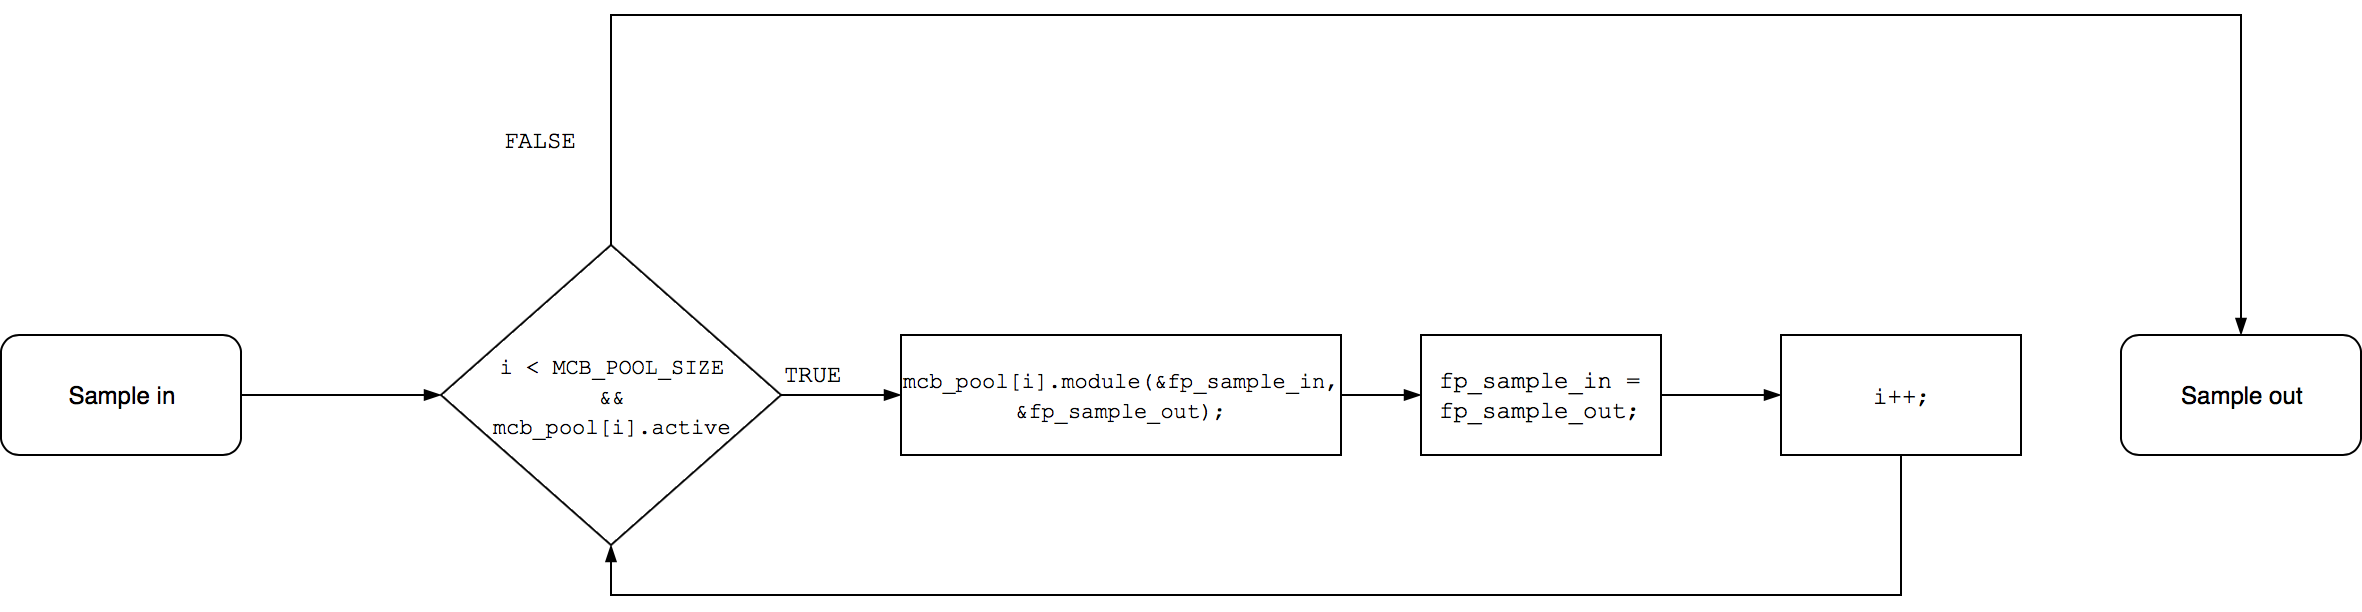
\includegraphics[width=\textwidth]{billeder/Flowchart_for_effektmoduler.png}
	\caption{Flowchart for iteration gennem effektmoduler}
	\label{fig:effektmoduler}
\end{figure}

På figur (\ref{fig:effektmoduler}) illustreres det, hvordan de enkelte moduler bliver kaldet, når de er aktiveret, efter hver sample kommer ind.
Grunden til at outputtet fra hver modul bliver sat til input, er at det ønskes at opnå en seriel kobling af effekterne.
%indsæt flowchart her når du er tilbage

\subsection{Generering af PWM-signal til DAC}
Timeren benyttes desuden til at generere et PWM-signal, hvis duty cycle er styret af timeren og resultatet af A/D konverteringen af indgangssignalet. 
\begin{wrapfigure}{r}{0.5\textwidth}
	\centering
	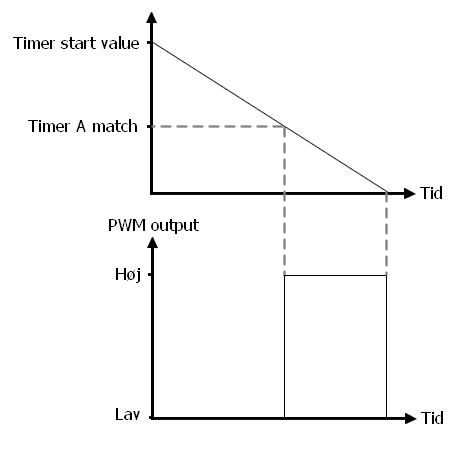
\includegraphics[width=0.5\textwidth]{billeder/timer3PWM.png}
	\caption{\label{fig:PWMfromtimer}Generering af PWM-signal ud fra timer. }
\end{wrapfigure}
Figur \ref{fig:PWMfromtimer} viser hvordan PWM-signalets duty cycle bliver bestemt af den værdi, som bliver gemt på Timer A's match register. 
Den værdi kommer fra den periodiske sampling af lydsignalet gennem ADC'en, hvor resultatet af hver sampling netop gemmes i match registeret. 
Således genskabes signalet som et digitalt PWM signal. 

\section{Genskabelse af signal via DAC igennem SPI}

\section{Håndtering af brugergrænseflade og human input interface}

\husk{Sonny}{Kan dette anvendes?}
%For at kunne anvende enheden skal enheden kunne udveksle nødvendige informationer med brugeren, input skal altså kunne modtages, her valgte gruppen at anvende en "drehimpulsgeber", og respons skal oplyses, her valgte gruppen et grafisk repræsenteret menu system.
For at kunne anvende enheden skal enheden kunne udveksle nødvendige informationer med brugeren. 
Input skal kunne modtages, her valgte gruppen at anvende en "drehimpulsgeber".
Respons skal oplyses, her valgte gruppen et grafisk repræsenteret menu system.
%En menu består en række valgmuligheder repræsenteret af elementer brugeren kan bladre igennem og vælge imellem.
En menu består af en række valgmuligheder repræsenteret af elementer brugeren kan bladre igennem og vælge imellem.
Et valg kan lede til yderligere valgmuligheder inden for den valgte kategori, disse kan så præsenteres i form af en ny menu.
Til at udføre denne funktion valgte gruppen at anvende linkede lister.\newline
\husk{Indsæt diagram af den linkede liste her}
%I eksemplet herunder ses en hovedmenu "Root Menu" som linker til sit første element "Master volume", vælger brugeren dette element kan volumen sættes, elementet linker også til næste element så brugeren kan skifte til det, her er der tale om "Echo" elementet som istedet for at have en funktion linker til en ny menu nemlig "Echo menu" som så linker til sin egen liste af menu punkter.
I eksemplet herunder ses en hovedmenu ''Root Menu`` som linker til sit første element ''Master volume``, vælger brugeren dette element kan volumen sættes.
Elementet linker også til næste element så brugeren kan skifte til det, her er der tale om ''Echo`` elementet som i stedet for at have en funktion linker til en ny menu nemlig ''Echo menu`` som så linker til sin egen liste af menu punkter.
%En "drehimpulsgeber" kan anvendes til at producere 3 forskellige typer af input, drej mod uret herefter kaldet "vr", drej med uret "hr" og click.
%Når et input  modtages af programmet lægges det i en input kø til systemet er klar til at modtage input, er der tale om et "vr" fremvises foregående element i menuen, på samme måde anvendes et "hr" input til at gå til næste element i menuen og et click anvendes til at vælge det det nuværende element.
Drehimpulsgeberen kan anvendes til at producere 3 forskellige typer af input, drej mod uret herefter kaldet ''vr``, drej med uret ''hr`` og click.
\husk{Indsæt UI state machine her}
Når et input  modtages af programmet lægges det i en input kø til systemet er klar til at modtage input. Er der tale om et ''vr`` fremvises foregående element i menuen, på samme måde anvendes et ''hr`` input til at gå til næste element i menuen og et click anvendes til at vælge det nuværende element.
